% \documentclass[aip,jcp,preprint,unsortedaddress,a4paper,onecolum]{revtex4-1}
\documentclass[aip,jcp,a4paper,reprint,onecolumn]{revtex4-1}
% \documentclass[aps,pre,twocolumn]{revtex4-1}
% \documentclass[aps,jcp,groupedaddress,twocolumn,unsortedaddress]{revtex4}

\usepackage[fleqn]{amsmath}
\usepackage{amssymb}
\usepackage[dvips]{graphicx}
\usepackage{color}
\usepackage{tabularx}
\usepackage{algorithm}
\usepackage{algorithmic}

\makeatletter
\makeatother

\newcommand{\recheck}[1]{{\color{red} #1}}
\newcommand{\redc}[1]{{\color{red} #1}}
\newcommand{\bluec}[1]{{\color{blue} #1}}
\newcommand{\vect}[1]{\textbf{\textit{#1}}}
\newcommand{\dd}[1]{\textsf{#1}}

\newcommand{\AT}{{\textrm{{AT}}}}
\newcommand{\EX}{{\textrm{EX}}}
\newcommand{\CG}{{\textrm{CG}}}
\newcommand{\HY}{{\Delta}}
\newcommand{\rdf}{{\textrm{rdf}}}



\begin{document}

\title{The reliability of AdResS as a way of
sampling the Grand-Canonical ensemble}
\author{Han Wang}
\affiliation{Institute for Mathematics, Freie Universit\"at Berlin, Germany}
\author{Carsten Hartmann}
\affiliation{Institute for Mathematics, Freie Universit\"at Berlin, Germany}
\author{Christof Sch\"utte}
\affiliation{Institute for Mathematics, Freie Universit\"at Berlin, Germany}
\author{Luigi Delle Site}
\affiliation{Institute for Mathematics, Freie Universit\"at Berlin, Germany}

\begin{abstract}
\end{abstract}

\maketitle

\section{Introduction}
% The Adaptive Resolution Simulation (AdResS) scheme~\cite{jcp,pre} is a
% method that increase the resolution in some spacial regions in the
% system, while keep the rest at lower resolution.
The Adaptive Resolution Simulation (AdResS) scheme~\cite{jcp,pre} is a
method that concurrently simulates a molecular system by different
resolutions in different spacial regions.  The word ``resolution''
means how much detail is included in a molecular model: the higher the
resolution, the model is more precise, and the more computational
effort is demanded, correspondingly.  The advantage is obvious: it
keeps track of both of the local fine-grained processes in the
high-resolution regions and the on-going large scale properties with a
much lower computational expense comparing to the system that, as a
whole, is described by the high-resolution model. The key feature of
AdResS is that it allows an on-the-fly changing of resolution when a
molecule travels from a high-resolution region to a low-resolution
region and vice versa. Moreover, recent research~\cite{prlgc, rdfcorr}
numerically demonstrates that different resolutions reach a
thermodynamic equilibrium as if the whole system is equilibriated
under the high-resolution description. Therefore, the a region with a
certain resolution exchanges molecules with the rest of the system in
a Grand-Canonical fashion. This work, from the theoretical point of
view, studies the conditions, under which the AdResS is an effective
Grand-Canonical simulation, and tries to shed light on the accuracy of
the sampling.

\section{A brief description of the AdResS scheme}

In this work, the higher resolution refers to the atomistic
description (AT) of a molecule, while the lower resolution refers to
the its coarse-grained (CG) modeling.  We assume the dynamics of the
system is subjected to the Langevin equation, which the thermostat
usually used in the AdResS simulations:
\begin{align}
  \dd d\vect r_i &= \vect v_i\dd dt\\
  m_i\dd d\vect v_i &= [-m_i\xi_i\vect v_i + \vect F_i]\,\dd dt + \sqrt{2\sigma_i}\,\dd d\vect W_t
\end{align}
where $\dd d\vect W_t$ is the standard Wiener process. We denote the
phase space variable $\vect x = \{\vect r_i, \vect v_i\}$. $\vect r_i,
\vect v_i$ are the degrees of freedoms (DOFs) of the system.  If the
system is conservative, namely $\vect F_i = -\nabla_{\vect r_i}U$,
then it is shown the equilibrium density distribution is $p(\vect
x)\propto e^{-\beta\mathcal H(\vect x)}$. In the AdResS scheme,
different resolutions in the system are described by a weighting
function of position $w(\vect r)$. Usually the higher resolutions is
denoted by $w = 1$, while the lower resolution is denoted by $w = 0$.
Between the higher and lower resolutions, a hybrid region allows a 
molecule has both the resolutions. The weighting function changes smoothly
from 0 to 1. A possible weighting function is:
\begin{align}\label{eqn:new-w}
  w(\vect r) =
  \left\{
    \begin{array}{lcl}
      1 &\quad& \chi < 0\\
      1  && 0 < \chi < r_c\\
      \cos^2\big[\frac{\pi}{2(d_{\HY} - r_c)} (\chi - d_{\textrm{ex}} - r_c)\big] && r_c < \chi < d_{\HY} \\
      0 &&  d_{\HY}  < \chi.
    \end{array}
  \right.
\end{align}
Where $\chi$ is the distance to the boundary of the higher resolution
region. $\chi < 0$ means the molecule is in the higher resolution
region.  $d_{\HY}$ is the thickness of the hybrid region. $r_c$ is the
cut-off radius.  The intermolecuar force is modeled by the following
interpolation formula:
\begin{align}
  \vect F_{\alpha\beta} =
  w_\alpha w_\beta\vect F^{\AT}_{\alpha\beta} +
  [1-w_\alpha w_\beta]\vect F^{\CG}_{\alpha\beta} +
  w_\alpha w_\beta (1-w_\alpha w_\beta)\vect F_{\alpha\beta}^{\rdf}.
\label{grf}
\end{align}
Where $ \vect F^{\AT}_{\alpha\beta}$, $ \vect F^{\CG}_{\alpha\beta}$
are the intermolecuar interaction of the atomistic and coarse-grained
resolutions, respectively.  $\vect F_{\alpha\beta}^{\rdf}$ is the RDF
correction force, and is determined by a TFI-IBI
loop~\cite{rdfcorr}. On top of this interpolation formula, a
thermodynamic force ${\vect F}^{\textrm{th}}$ is applied to ensure the
right equilibrium between the resolutions:
\begin{equation}
  {\vect F}_{\alpha}=
  \sum_{\beta}{\vect F}_{\alpha\beta}+
  {\vect F}^{\textrm{th}}(\vect r_\alpha).
\label{mody}
\end{equation}
which is defined by
\begin{equation}
  p_{\AT}+
  \frac{\rho_{0}}{M_\alpha}
  \int_{\Delta} {\vect F}^\text{th}(\vect r)\,\dd d\vect r
  =p_{\CG}
  \label{thf}
\end{equation}
In practice, the thermodynamic force is determined by a iterative
scheme.  For details we refer readers to Ref.~\cite{prlgc}. Notice the
AdResS system is not Hamiltonian~\cite{presolo,prlcomm}, however, by
freezing the DOFs in the hybrid region, the atomistic and
coarse-grained regions are Hamiltonian. This gives rise to the basic
idea of the present study.

\section{Theoretical considerations}
\subsection{The outline of the basic idea}
Here we denote the degrees of freedoms and number of particles in the
atomistic region (AT), hybrid region ($\HY$) and the coarse-grained
region (CG) by $(\vect x_1, N_1)$, $(\vect x_2, N_2)$ and $(\vect x_3,
N_3)$, respectively. Therefore, the target is to prove the atomistic
region is subject to the Grand-Canonical ensemble: 
\begin{align}
  p(\vect x_1, N_1) = \frac{1}{\mathcal Q_1}
  e^{\beta\mu_{\AT} N_1 - \beta \mathcal H_{N_1}^{\AT}(\vect x_1)} 
\end{align}
where the partition function $\mathcal Q_1$ is defined by
\begin{align}
  \mathcal Q_1 =
  \sum_{N_1}\int
  \dd d\vect x\,
  e^{\beta\mu_{\AT} N_1 - \beta \mathcal H_{N_1}^{\AT}(\vect x_1)}
\end{align}
The marginal probability of finding $N_1$ molecules in the
AT region is:
\begin{align}\label{eqn:p-2}
  p(N_1) = \int\dd d\vect x_1\, p(\vect x_1, N_1)
  =
  \frac{1}{\mathcal Q_1}e^{\beta\mu_{AT} N_1}Q_{N_1}
\end{align}
where $Q_{N_1}$ is the partition function for a canonical ensemble
with $N_1$ atomistic molecules:
\begin{align}
  Q_{N_1}  =
  \int\dd d\vect x_1\,
  e^{ - \beta \mathcal H_{N_1}^{\AT}(\vect x_1)}
\end{align}
Let us consider:
\begin{align}
  p(\vect x_1, N_1) = p(\vect x_1 | N_1)\,p(N_1)
\end{align}
Rigorously speaking, for a truly Grand-Canonical ensemble,
the conditional probability $p(\vect x_1 | N_1)$ 
should be
\begin{align}\label{eqn:p-1}
  p(\vect x_1 | N_1) &= \frac{1}{Q_{N_1}} e^{-\beta \mathcal H_{N_1}^{AT}(\vect x_1)} \end{align}
It must be kept in mind that we always compare the distributions of the AdResS simulation
with a those of a full atomistic reference system, which is ideally divided
in subregions corresponding to the AT, $\HY$ and CG regions of the AdResS
simulation. The first step in our procedure is to fix the number of molecules in the atomistic
region and consider the conditional probability $p(\vect x_1 |
N_1)$. If the AdResS set up, leads to the Grand-Canonical ensemble, this
probability should be the same as the corresponding one of a full
atomistic reference system, namely Eqn.~\eqref{eqn:p-1} (natual Grand-Canonical).  Then, if the
probability of finding $N_1$ molecules in the atomistic region is also
the same as the full atomistic reference system, namely
Eqn.~\eqref{eqn:p-2}, we can safely state that the atomistic region of AdResS
samples configurations in a Grand Canonical fashion.


\subsection{The probability $p(\vect x_1 | N_1)$}
To prove the statement above, the probability $p(\vect x_1 | N_1)$ is divided into two parts:
\begin{align}\label{eqn:divide-cond-p}
  p(\vect x_1 | N_1) = \sum_{N_2}\int
  p(\vect x_1 | N_1; \vect x_2, N_2) \,
  p(\vect x_2, N_2 | N_1)
  \,\dd d\vect x_2
\end{align}
$p(\vect x_1 | N_1; \vect x_2, N_2)$ is the probability obtained by fixing the
coordinates and number of particles in the region $\HY$ and considering
the distribution of the DOFs in the AT region. As we have shown before,
if we modify the weighting function by Eqn.~\eqref{eqn:new-w}
We can prove:
\begin{align}
  p(\vect x_1 | N_1; \vect x_2, N_2)
  \propto &\,
  e^{-\beta\mathcal H_{N_1}^{\AT}(\vect x_1; \vect x_2, N_2)}
\end{align}
with an atomistic Hamiltonian:
\begin{align}
  \mathcal H_{N_1}^{{\AT}}(\vect x_1; \vect x_2, N_2) = &\,
  \sum_{j=1}^{N_1}\frac12 m_i\vect v_i^2 + 
  \sum_{i,j=1}^{N_1}\frac12 U^{{\AT}}(\vect r_i - \vect r_j)  +
  \sum_{i=1}^{N_1}\sum_{j=N_1+1}^{N_2} U^{{\AT}}(\vect r_i - \vect r_j)   
\end{align}
which is exactly the same as the full atomistic reference system.
Here are some remarks on this argument:
\begin{enumerate}\itemsep -1pt
\item All interactions in the system are short-range cut-offed (the
  electrostatic interaction is treated by the reaction field method),
  so that the AT region does NOT interacting with the CG region.
\item The number of molecules and their coordinates are assumed to be
  fixed in the $\HY$ region.  Under this assumption, we firstly study
  the conditional probability $p(\vect x_1 | N_1; \vect x_2, N_2)$ of
  the AT region embedded in the fixed $\HY$ environment, and then count
  all possible realizations of the $\HY$ region, which is subject to
  the distribution $p(\vect x_2, N_2 | N_1)$.
  Eqn.~\eqref{eqn:divide-cond-p} validates this two-stage approach of
  investigating $p(\vect x_1 | N_1)$.
\item Due to the point 2, the correlation between the molecules
  in $\HY$ and CG regions are not important in our argument, because
  the DOFs in the $\HY$ region are fixed anyway.
\end{enumerate}

\noindent
At this point, the key question is that whether the probability in the $\HY$ region, $p(\vect
x_2, N_2 | N_1)$ is the same as that of the full atomistic reference
system. Generally, this seems not be the case, but it is possible to
derive necessary conditions to this aim. The simplest ones involve
the marginal distribution functions, namely
\begin{align}
  \rho_{\HY}(\vect r) &= \rho_{\AT}(\vect r)\\
  g_{\HY}( r) &= g_{\AT}(r)
\end{align}
The first order marginal distribution is the particle (or molecular) density 
$\rho_{\HY}(\vect r)$, while the second order marginal distribution is
the radial distribution function (RDF), $g_{\HY}(r)$. The necessary
conditions are that these two distribution should be the same as those of the fully atomistic reference system.


\subsection{Discussion about the thermodynamic force}
\begin{figure}
  \centering
  \begin{minipage}[t]{0.49\linewidth}
  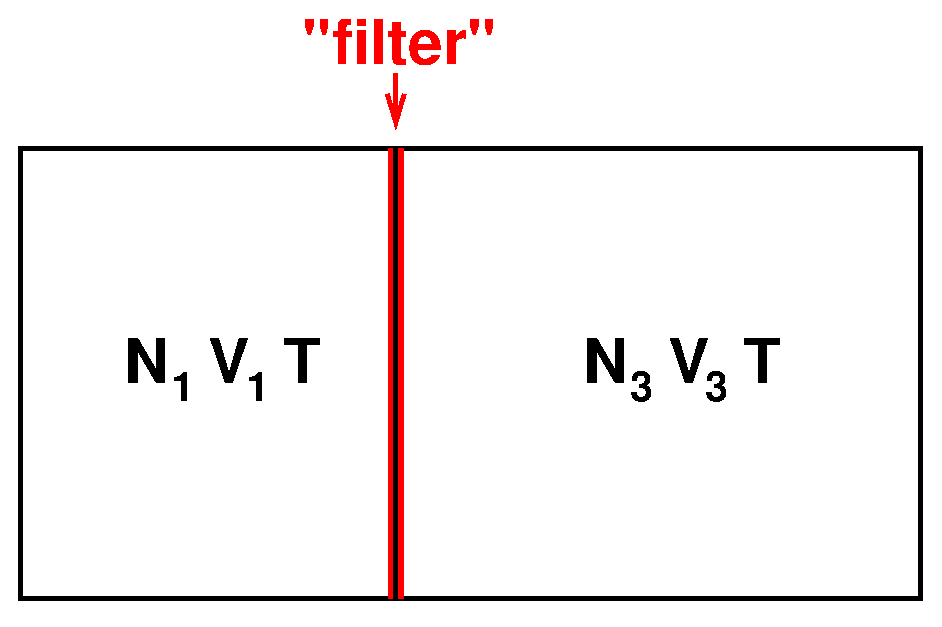
\includegraphics[width=0.6\textwidth]{fig.grand/partition.eps}    
  \end{minipage}
  % \begin{minipage}[t]{0.49\linewidth}
  % 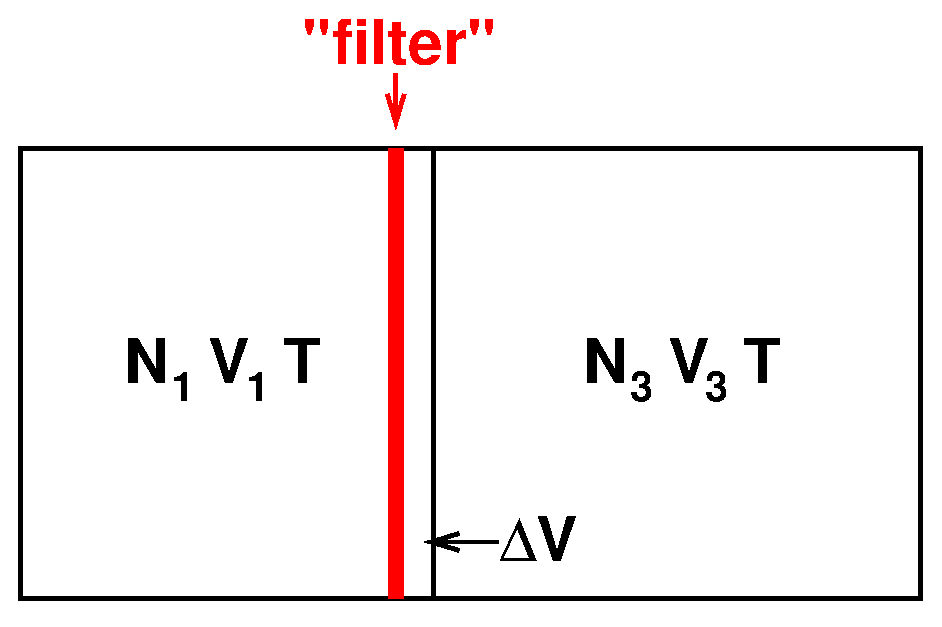
\includegraphics[width=0.6\textwidth]{fig.grand/partition-1.eps}    
  % \end{minipage}
  \caption{Schematic plot of the AdResS system in thermodynamic equilibrium}
  \label{fig:tmp1}
\end{figure}
Here, two assumptions are made:
\begin{enumerate}\itemsep -1pt
\item $N_2\ {\ll}\ N_1 \ll N_3$: the second inequality corresponds to
  the thermodynamic limit of the Grand-Canonical ensemble. The first
  one actually assumes that the $\HY$ region is infinitely thin so that it
  can be viewed as an infinitesimal membrane that allows free exchange of molecules from
  the AT region to the CG region and vice versa.
\item We now define a supplementary Hamiltonian:
  \begin{equation}
    \mathcal H(\vect x_1, N_1; \vect x_3, N_3) =
    \mathcal H_{N_1}^{\AT}(\vect x_1) + \mathcal H_{N_3}^{\CG}(\vect x_3); 
  \end{equation}
  The condition above is true, in the thermodynamic limit, if the system is
  short-range correlated.
\end{enumerate}
The equilibrium in the AT and CG region is assured by the membrane $\HY$ via the thermodynamic force. Conceptually, we assume there is an infinitely thin
``filter'' (see Fig.~\ref{fig:tmp1}) located at the interface between
the AT and CG regions. When a molecule travels from the CG region to
the AT region, the filter does some work $\omega_0$ on the system.
Therefore, we add an empirical term in the Hamiltonian of the system
$N_1\omega_0$, which denotes the work done by the thermodynamic force.
% \recheck{
%   Actually, here, it is better to argue in this way:
%   $w_0$ can be the work of any force, not necessarily thermodynamics force,
%   because here we do not put any special condition on $w_0$.
%   It is simply ``the work done by the filter'' and can be any value.
%   It is important to notice
%   an arbitrary $w_0$ can also ensure an equilibrium between
%   the AT and CG region, but this equilibrium is generally
%   wrong, i.e. $\rho_{\AT}\neq \rho_{\CG} \neq \rho_0$.
%   But anyway we can prove the under this equilibrium (which may be
%   wrong), the chemical potential difference between the AT and
%   CG regions is the work $w_0$.
% }
Having fixed the number of molecules in the three regions, and by following the
arguments of the last section, both the AT and the CG regions are
subject to the Boltzmann distribution.
Thus, the fixed-number partition function of the system reads
\begin{align}\nonumber
  q(N,V,T)
  &= \frac1{N!}\int
  \dd d\vect x
  e^{-\beta
    [\mathcal H(\vect x_1, N_1; \vect x_3, N_3) +
    N_1\omega_0]}\\\nonumber
  &= \frac1{N!}\int
  \dd d\vect x_1\dd d\vect x_3\,
  e^{-\beta
    [\mathcal H_{N_1}^{\AT}(\vect x_1) +
    \mathcal H_{N_3}^{\CG}(\vect x_3) +
    N_1\omega_0]}\\\nonumber
  & = \frac{N_1!N_3!}{N!}
  e^{-\beta N_1\omega_0}
  \frac{1}{N_1!}\int\dd d\vect x_1 e^{-\beta\mathcal H_{N_1}^{\AT}(\vect x_1)}
  \frac{1}{N_3!}\int\dd d\vect x_3 e^{-\beta\mathcal H_{N_3}^{\CG}(\vect x_3)}\\
  & = \frac{N_1!N_3!}{N!}
  e^{-\beta N_1\omega_0}
  Q_{\AT}(N_1, V_1, T)\,
  Q_{\CG}(N_3, V_3, T) 
\end{align}
Considering the permutations of particles, the number of possibilities of
$N_1$ molecules being in the atomistic region and $N_3$ molecules being
in the coarse-grained region is  $\frac{N!}{N_1!N_3!}$.
Therefore, the partition function of the whole system reads
\begin{align}\nonumber
  Q(N,V,T) &= \sum_{N_1}
  \frac{N!}{N_1!N_3!} \frac{N_1!N_3!}{N!}
  e^{-\beta N_1\omega_0}
  Q_{\AT}(N_1, V_1, T)\,
  Q_{\CG}(N_3, V_3, T) \\
  &= \sum_{N_1}
  e^{-\beta N_1\omega_0}
  Q_{\AT}(N_1, V_1, T)\,
  Q_{\CG}(N_3, V_3, T) 
\end{align}
with natural relations:
\begin{align}
  N &= N_1 + N_3\\
  V &= V_1 + V_3
\end{align}
It can be proved that (see for example
Ref.~\cite{tuckeman2010statistical}) if
\begin{align}\label{eqn:condition}
  -\beta \bar N_1\omega_0 +
  \ln Q_{\AT}(\bar N_1, V_1, T) + \ln Q_{\CG}(N - \bar N_1, V_3, T) \gg \ln N 
\end{align}
where
\begin{align}
  \bar N_1 = \underset{N_1}{\textrm{argmax}}\:
  e^{-\beta N_1\omega_0}
  Q_{\AT}(N_1, V_1, T) \,Q_{\CG}(N - N_1, V_3, T)
\end{align}
then
\begin{align}
  \ln Q(N, V, T)
  \approx
  -\beta \bar N_1\omega_0 + 
  \ln Q_{\AT}(\bar N_1, V_1, T) + \ln Q_{\CG}(N - \bar N_1, V_3, T)
\end{align}
or equivalently
\begin{align}\label{eqn:a-energy-1}
  A(N, V, T)
  \approx
  \bar N_1\omega_0 +
  A_{\AT}(\bar N_1, V_1, T) + A_{\CG}(N - \bar N_1, V_3, T)
\end{align}
Where $A$ denotes the Helmhotz free energy.  $\bar N_1$ is the maximum
parameter of $e^{-\beta N_1\omega_0} Q_{\AT}(N_1, V_1, T) \,Q_{\CG}(N - N_1,
V_3, T)$.
The crucial question is if the condition~\eqref{eqn:condition}
is satisfied. Generally this is true: $Q_{\CG}(N - \bar N_1, V_3, T)$
is proportional to the free energy $A_{\CG}(N - \bar N_1, V_3, T)$,
which is an extensive thermodynamic variable, so
$A_{\CG}(N - \bar N_1, V_3, T)$ is proportional to $N-\bar N_1$.
Due to the thermodynamic limit $N \gg \bar N_1$,
$A_{\CG}(N - \bar N_1, V_3, T)$ is actually proportional $N$, which
is much larger than $\ln N$ under thermodynamic limit. This
validates condition~\eqref{eqn:condition}.
We will see later that this maximum corresponds to the maximum
value of probability $p(N_1)$; this is also the equilibrium molecular
number in the AT region under the thermodynamic limit.  Since $\bar
N_1$ is the maximum, by differentiating on the right hand side of
Eqn.~\eqref{eqn:a-energy-1}, we have the relation:
\begin{align}
  \omega_0 = \mu_{\CG}(N - \bar N_1, V_3, T)  - \mu_{\AT}(\bar N_1, V_1, T)
\end{align}
That means that the difference in the chemical potential between the AT and CG
regions is taken care by the thermodynamic force.
If the thermodynamic force ensures an
equilibrium that is the same as the full atomistic reference system,
the work should be the same as the
chemical potential difference between the atomistic and coarse-grained
resolutions, namely
\begin{align}\label{eqn:w-mu-diff}
  \omega_0 = \mu_{\CG}(\rho_0V_3, V_3, T) - \mu_{AT}(\rho_0 V_1, V_1, T)
\end{align}
$\rho_0$ is the density at which the atomistic and coarse-grained
resolutions should match,
namely $\bar N_1 = \rho_0V_1$ and $N - \bar N_1 = \rho_0(V - V_1)$ should apply.
% \recheck{As we mentioned before, the work done by the filter
%   can be arbitrary, and may lead to a wrong equilibrium.
%   To ensure a right equilibrium, the necessary condition for
%   ``the work done by the filter'' is that it is the same
%   as the chemical potential difference between the
%   atomistic and coarse-grained resolutions. (Notice, the
%   conception is different from ``the chemical potential difference between
%   the AT and CG regions''. We should keep in mind this
%   difference to understand the argument correctly.
% }
Eqn.~\eqref{eqn:w-mu-diff} is a necessary
condition for the thermodynamic force that ensures
the correct equilibrium of the AT and CG regions.\\

\noindent
Now we translate from the language of Helmhotz free
energy into that of the grand potential.
Under the thermodynamic limit, they are the same.
Assuming the system reaches an
equilibrium of flat density profile of $\rho_0$ all over the AdResS simulation box, 
Eqn.~\eqref{eqn:a-energy-1} becomes:
\begin{align}\label{eqn:g-energy-1}
  G(\mu, V, T) \approx
  \rho_0V_1\omega_0
  + G_{\AT}(\mu_{\AT}, V_1, T) + G_{\CG}(\mu_{\CG}, V - V_1, T)
\end{align}
where
\begin{align}
  G(\mu, V, T) = A(N, V, T) - \mu_{\AT} \bar N_1 - \mu_{\CG}(N - \bar N_1)
\end{align}
Because of the equilibrium situation, the derivative of r.h.s. of
Eqn.~\eqref{eqn:g-energy-1} with respect to atomistic volume $V_1$
should vanishes (the same argument as the Helmhotz free energy):
\begin{align}
  \rho_0\omega_0 = -p_{\AT}+p_{\CG} \quad\Longrightarrow\quad
  p_{\AT} + \rho_0\omega_0 = p_{\CG}
\end{align}
which is exactly the definition of the thermodynamic force.
This is another necessary condition for the
thermodynamic force, which is actually satisfied by the definition of it,
namely Eqn.~\eqref{thf}.
% \begin{equation}
%   p_{\AT}+
%   \frac{\rho_{0}}{M_\alpha}
%   \int_{\Delta} {\vect F}^\text{th}(x)\,\dd dx
%   =
%   p_{\CG}
% \label{thf}
% \end{equation}
% \recheck{
%   This is an other necessary condition that ``the work
%   done by the filter'' ensures a right equilibrium.
%   Surprisingly, this necessary condition is exactly fitted
%   by the definition of the ``thermodynamic force''.
% }

\subsection{The number probability $p(N_1)$}
Now let us consider the marginal distribution $p(N_1)$
\begin{align}\nonumber
  p(N_1)
  % &=
  % \int
  % \dd d\vect x
  % \,e^{-\beta
  %   [\mathcal H(\vect x_1, N_1; \vect x_3, N_3) +
  %   N_1\omega_0]}\\\nonumber
  &=
  \frac{N!}{N_1!N_3!}
  \int
  \dd d\vect x_1\dd d\vect x_3  \:
  \frac{1}{Q(N,V,T) N!}
  e^{-\beta
    [\mathcal H_{N_1}^{\AT}(\vect x_1) +
    \mathcal H_{N_3}^{\CG}(\vect x_3) +
    N_1\omega_0]}\\\nonumber
  &=
  \frac{N!}{N_1!N_3!}
  \frac{N_1!N_3!}{Q(N,V,T) N!}
  e^{-\beta N_1\omega_0}
  \bigg[
  \frac1{N_1!}
  \int
  \dd d\vect x_1
  e^{-\beta \mathcal H_{N_1}^{\AT}(\vect x_1)}
  \bigg]
  \bigg[
  \frac1{N_3!}
  \int
  \dd d\vect x_3
  e^{-\beta \mathcal H_{N_3}^{\CG}(\vect x_3)}
  \bigg]  \\\nonumber
  &=
  \frac
  {
    e^{-\beta N_1\omega_0}
    Q_{\AT}(N_1,V_1,T) Q_{\CG}(N-N_1,V_3,T)
  }
  {
    \sum_{n_1}
    e^{-\beta n_1\omega_0}
    Q_{\AT}(n_1,V_1,T) Q_{\CG}(N-n_1,V_3,T)
  }
\end{align}
where $n_1$ is the summation variable that goes from 0 to $N$,
however, when $n_1$ is not much smaller than $N$ (i.e. out of the range of the
thermodynamic limit), the statistic is only of marginal importance,
and can be neglected safely.
The atomistic marginal distribution, which the AdResS simulation should
reproduce is
\begin{align}
  p_{\AT}(N_1)
  &=
  \frac
  {
    Q_{\AT}(N_1,V_1,T) Q_{\AT}(N-N_1,V_3,T)
  }
  {
    \sum_{n_1}
    Q_{\AT}(n_1,V_1,T) Q_{\AT}(N-n_1,V_3,T)
  }  
\end{align}
We want to calculate the difference between $p(N_1)$ and $p_{\AT}(N_1)$.
By multiplying the numerator of $p(N_1)$ by the denominator of
$p_{\AT}(N_1)$ (denoted by $T_1$),
and multiplying the numerator of $p_{\AT}(N_1)$
by the denominator of $p(N_1)$ (denoted by $T_2$), we have
\begin{align}
  T_1
  &=
  e^{-\beta N_1\omega_0}
  Q_{\AT}(N_1,V_1,T) Q_{\CG}(N-N_1,V_3,T)
  \times
  \sum_{n_1}
  Q_{\AT}(n_1,V_1,T) Q_{\AT}(N-n_1,V_3,T)\\
  T_2
  &=
  Q_{\AT}(N_1,V_1,T) Q_{\AT}(N-N_1,V_3,T)
  \times
  \sum_{n_1}
  e^{-\beta n_1\omega_0}
  Q_{\AT}(n_1,V_1,T) Q_{\CG}(N-n_1,V_3,T)
\end{align}
The difference between $T_1$ and $T_2$ is basically the difference
between $p(N_1)$ and $p_{\AT}(N_1)$.
Calculating $T_1$:
\begin{align}\nonumber
  T_1
  &=
  \sum_{n_1}
  e^{-\beta N_1\omega_0}
  Q_{\AT}(n_1,V_1,T)\,
  Q_{\AT}(N_1,V_1,T)\,
  Q_{\AT}(N-n_1,V_3,T)\,
  Q_{\CG}(N-N_1,V_3,T) \\\nonumber
  &=
  \sum_{n_1}
  \exp
  \big\{-\beta
  \big[
  \omega_0N_1 +
  A_{\AT}(n_1,V_1,T) +
  A_{\AT}(N_1,V_1,T) +
  A_{\AT}(N-n_1,V_3,T) +
  A_{\CG}(N-N_1,V_3,T)
  \big]
  \big\}
\end{align}
Since we work under the hypothesis that the atomistic region is much smaller than the whole system, it
is reasonable to assume $n_1 \ll N$ nad $N_1\ll N$. We have the following
expansions:
\begin{align}
  A_{\AT}(N-n_1,V_3,T)
  &=
  A_{\AT}(N,V_3,T)
  - \mu_{\AT}\,n_1
  + \frac12 \kappa_{\AT}\,n_1^2 + \textrm{h.o.t.} \\
  A_{\CG}(N-N_1,V_3,T)
  &=
  A_{\CG}(N,V_3,T)
  - \mu_{\CG}\,N_1
  + \frac12 \kappa_{\CG}\,N_1^2 + \textrm{h.o.t.}
\end{align}
One should keep in mind the conditions:
\begin{align}\label{eqn:mu-eq}
  \mu_{\CG} &= \mu_{\AT} + \omega_0\\\label{eqn:kappa-eq}
  \kappa_{\CG} &= \kappa_{\AT}
\end{align}
We have $T_1$
\begin{align}\nonumber
  T_1
  = \,&
  \sum_{n_1}
  \exp
  \big\{-\beta
  \big[
  A_{\AT}(n_1,V_1,T) +
  A_{\AT}(N_1,V_1,T) +
  A_{\AT}(N,V_3,T) +
  A_{\CG}(N,V_3,T) \\
  \,&-
  \mu_{\AT}\,(N_1 + n_1) +
  \frac12 \kappa_{\AT}(N_1^2 + n_1^2) +
   \textrm{h.o.t.}
  \big]
  \big\}
\end{align}
% Similarly, multiplying the numerator of $p_{\AT}(N_1)$ by the denominator of
% $p(N_1)$, we have the term denoted by $T_2$
Similarly, we calculate $T_2$:
\begin{align}\nonumber
  T_2
  &=
  \sum_{n_1}
  e^{-\beta n_1\omega_0}
  Q_{\AT}(n_1,V_1,T)\,
  Q_{\AT}(N_1,V_1,T)\,
  Q_{\CG}(N-n_1,V_3,T)\,
  Q_{\AT}(N-N_1,V_3,T) \\\nonumber
  &=
  \sum_{n_1}
  \exp
  \big\{-\beta
  \big[
  \omega_0n_1 +
  A_{\AT}(n_1,V_1,T) +
  A_{\AT}(N_1,V_1,T) +
  A_{\CG}(N-n_1,V_3,T) +
  A_{\AT}(N-N_1,V_3,T)
  \big]
  \big\}
\end{align}
with similar expansions and by the conditions Eqn.~\eqref{eqn:mu-eq}
and \eqref{eqn:kappa-eq}, we have:
\begin{align}\nonumber
  T_2
  = \,&
  \sum_{n_1}
  \exp
  \big\{-\beta
  \big[
  A_{\AT}(n_1,V_1,T) +
  A_{\AT}(N_1,V_1,T) +
  A_{\AT}(N,V_3,T) +
  A_{\CG}(N,V_3,T) \\
  \,&-
  \mu_{\AT}\,(N_1 + n_1) +
  \frac12 \kappa_{\AT}(N_1^2 + n_1^2) +
   \textrm{h.o.t.}
  \big]
  \big\}
\end{align}
Therefore, term $T_1$ and $T_2$ are consistent with  the second leading
order, which means $p(N_1)$ is a good approximation of $p_{\AT}(N_1)$
to the second leading order.



\section*{References}
\bibliography{ref}{}
\bibliographystyle{unsrt}





\end{document}